% !TeX spellcheck = pl_PL
\documentclass[12pt]{oska}

% Lista wszystkich języków stanowiących języki pozycji bibliograficznych użytych w pracy.
% (Zgodnie z zasadami tworzenia bibliografii każda pozycja powinna zostać utworzona zgodnie z zasadami języka, w którym dana publikacja została napisana.)
\usepackage[english,polish]{babel}

% Użyj polskiego łamania wyrazów (zamiast domyślnego angielskiego).
\usepackage{polski}

\usepackage[utf8]{inputenc}

% dodatkowe pakiety
\usepackage{mathtools}
\usepackage{amsfonts}
\usepackage{amsmath}
\usepackage{amsthm}
\usepackage{bm}
\usepackage{adjustbox}
\usepackage[dvipsnames]{xcolor}
\usepackage{textcomp}

% obrazki
\usepackage{graphicx}
\usepackage{rotating}
\usepackage{caption}
\usepackage{float}

% --- < bibliografia > ---

\usepackage{placeins}	% poprawia float

\let\Oldsection\section
\renewcommand{\section}{\FloatBarrier\Oldsection}

\let\Oldsubsection\subsection
\renewcommand{\subsection}{\FloatBarrier\Oldsubsection}

\let\Oldsubsubsection\subsubsection
\renewcommand{\subsubsection}{\FloatBarrier\Oldsubsubsection}

\usepackage[
style=numeric,
sorting=none,
% Zastosuj styl wpisu bibliograficznego właściwy językowi publikacji.
language=autobib,
autolang=other,
% Zapisuj datę dostępu do strony WWW w formacie RRRR-MM-DD
%urldate=iso,
%seconds=true,
% Nie dodawaj numerów stron, na których występuje cytowanie
backref=false,
% Podawaj ISBN.
isbn=true,
% Nie podawaj URL-i, o ile nie jest to konieczne
url=false,
% Ustawienia związane z polskimi normami dla bibliografii
maxbibnames=6,
minbibnames=6,
% Jeżeli używamy Bibera:
backend=biber
]{biblatex}

\AtBeginBibliography{
\renewcommand\labelnamepunct{:\space}
\renewcommand\newunitpunct{\addcomma\space}
\renewcommand{\finentrypunct}{}

\renewcommand{\bibopenparen}{\addcomma\addspace}
\renewcommand{\bibcloseparen}{\addspace}
}

\usepackage{csquotes}
% Ponieważ `csquotes` nie posiada polskiego stylu, można skorzystać z mocno zbliżonego stylu chorwackiego.
\DeclareQuoteAlias{croatian}{polish}

% Przecinki do numerów
\usepackage{icomma}
% ------------------------

% --- < listingi > ---

% Użyj czcionki kroju Times.
\usepackage{newtxtext}

\usepackage{listings}
\lstloadlanguages{TeX}

\lstset{
	literate={ą}{{\k{a}}}1
           {ć}{{\'c}}1
           {ę}{{\k{e}}}1
           {ó}{{\'o}}1
           {ń}{{\'n}}1
           {ł}{{\l{}}}1
           {ś}{{\'s}}1
           {ź}{{\'z}}1
           {ż}{{\.z}}1
           {Ą}{{\k{A}}}1
           {Ć}{{\'C}}1
           {Ę}{{\k{E}}}1
           {Ó}{{\'O}}1
           {Ń}{{\'N}}1
           {Ł}{{\L{}}}1
           {Ś}{{\'S}}1
           {Ź}{{\'Z}}1
           {Ż}{{\.Z}}1,
	basicstyle=\footnotesize\ttfamily,
}

% ------------------------

\AtBeginDocument{
	\renewcommand{\tablename}{\textbf{Tabela}}
	\renewcommand{\figurename}{\textbf{Rysunek}}
}

% ------------------------
% --- < tabele > ---

\usepackage{array}
\usepackage{tabularx}
\usepackage{multirow}
\usepackage{booktabs}
\usepackage{makecell}
\usepackage[flushleft]{threeparttable}

% defines the X column to use m (\parbox[c]) instead of p (`parbox[t]`)
\newcolumntype{C}[1]{>{\hsize=#1\hsize\centering\arraybackslash}X}

\setlength{\cftsecnumwidth}{10mm}
\setcounter{secnumdepth}{4}
\brokenpenalty=10000\relax

% ------------------------
% --- < do tego artykułu > ---
\sisetup{binary-units=true}
\DeclareSIUnit{\inch}{"}
\usepackage{import}

%---------------------------------------------------------------------------

\titlePL{Wielokanałowy system syntezy pola akustycznego}
\titleEN{Multichannel wave field synthesis system}
\affiliation{Akademia Górniczo-Hutnicza im. Stanisława Staszica w Krakowie}

%------------------------------------AUTORZY-----------------------

\namem{Marcel}
\surnamem{Piszak}
\email{marcel.piszak@gmail.com} % adres do korespondencji -- zazwyczaj głównego autora

% Jeśli jesteś jedynym autorem pracy - pozostaw poniższe pola puste

\namei{Szymon}
\surnamei{Mikulicz}

\nameii{Teresa}
\surnameii{Makuch}

\nameiii{Michał}
\surnameiii{Kmiecik}

\nameiiii{}
\surnameiiii{}

\nameiiiii{}
\surnameiiiii{}

%--------------------------STRESZCZENIE------------------------

\summaryPL{%
  Projekt obejmuje stworzenie systemu Wave Field Synthesis (WFS) opartego na
  macierzy głośników oraz komputerach Raspberry Pi. Rozwój tej technologii
  pozwala na osiągnięcie wrażeń przestrzennych niezależnych od punktu odsłuchu.
  Głośniki zawarte w macierzy, poprzez zastosowanie odpowiedniego przetwarzania
  sygnałów wejściowych, są w stanie formować kształt czoła fali akustycznej w
  taki sposób, aby kreować pozorne źródło dźwięku. Modułowość konstrukcji pozwala
  na jednoczesne niezależne przetwarzanie dużej liczby sygnałów oraz wysyłanie
  ich do poszczególnych kanałów. Jednocześnie umożliwia to  rozszerzanie systemu
  o kolejne macierze głośników, dzięki czemu możliwa jest dokładniejsza synteza
  pola akustycznego.
}

\summaryEN{
  The project consists of creating Wave Field Synthesis (WFS) system, that is
  based on a loudspeaker matrix and Raspberry Pi computers. Development of this
  technology allows to achieve spatial impressions that do not depend on the
  listener's position. Loudspeakers that are in the matrix, through the use of
  appropriate input signal processing, can create the shape of the acoustic
  wave in such a way, that a virtual sound source is created. Modularity of the
  design allows for simultaneous independent processing of big amount of signals
  and sending them to appropriate channels. This allows to extend the system
  with subsequent arrays of loudspeaker, for a better wave field synthesis
  capabilities.
}

%---------------------------------------------------------
% Nazwa pliku z bibliografią
%---------------------------------------------------------
\addbibresource{bibliografia.bib}


\begin{document}

\maketitles

\section{Wstęp}

Reprodukcja dźwięku jest bardzo szerokim zagadnieniem akustyki. W obecnych
czasach istnieje wiele technik pozwalających na odtworzenie panujących w
wybranym miejscu warunków akustycznych w zgoła innym otoczeniu. Złożoność
zjawisk związanych z propagacją fali akustycznej w rzeczywistym środowisku
sprawia, że omawiane zagadnienie staję się złożonym problemem. Jedną z
najistotniejszych trudności napotykanych podczas projektowania systemu
reprodukcji dźwięku jest ograniczenie przestrzeni dokładnego odwzorowania do
punktu, a właściwie niewielkiego obszaru wokół niego (tzw. \textit{sweet spot}).
Istnienie takiego ograniczenia wyklucza zastosowanie takich systemów w
sytuacjach, gdy mamy do czynienia z odbiornikiem wykonującym ruch w strefie
odsłuchu. Z pomocą przychodzą jednak systemy syntezy pola akustycznego (ang. \textit{Wave
Field Synthesis} -- WFS), które bazując na dużej liczbie głośników są w stanie
imitować fale akustyczne generowane przez źródła usytuowane nawet w dużej
odległości oraz będące w ruchu, ale co najważniejsze nie ograniczają strefy
odsłuchu do punktu. Obecnie istnieją różne warianty systemów WFS, projektowane
często z myślą o konkretnym zastosowaniu. 

Celem niniejszej pracy
było zaprojektowanie modułowego systemu syntezy pola akustycznego, opartego na
łatwo dostępnych komponentach i umożliwiającego stosunkowo prostą adaptację do
wybranego zastosowania.

\section{Synteza pola akustycznego}

Metoda WFS oparta jest na zasadzie Huygensa: każdy punkt
do którego dociera fala akustyczna staje się źródłem nowej fali. Ta zasada
jest zaimplementowana poprzez konstrukcję macierzy głośników, gdzie każdy z nich
jest punktem do którego dotarła fala akustyczna wyemitowana przez wirtualne
źródło dźwięku, przekazując falę dalej, a w praktyce tworząc ją, co pokazuje rysunek
\ref{r:Huygens}.

\begin{figure}[!tbh]
  \centering
  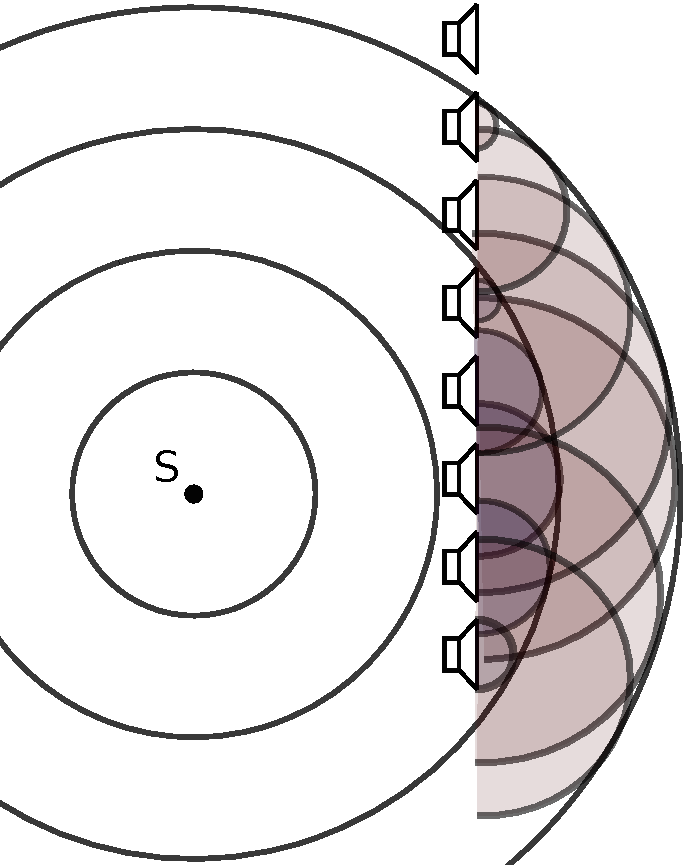
\includegraphics[scale=.4]{vecgraphics/WFS_idea.pdf}
  \caption{Zastosowanie zasady Huygensa w WFS: każdy głośnik jest punktem do
    którego dociera fala wyemitowana przez wirtualne źródło -- nowym źródłem
  dźwięku}
  \label{r:Huygens}
\end{figure}

Podstawowym równaniem w WFS jest całka Helmholtza-Huygensa (lub całka
Kirchoffa-Helmholtza), analityczna metoda liczenia rozkładu pola
akustycznego, która pozwala wyznaczyć ciśnienie akustyczne pochodzące od danego zestawu
źródeł w każdym punkcie zdefiniowanej przestrzeni~\cite{snaka}. Jest używana do
zdefiniowania funkcji opisującej ciśnienie akustyczne w pozycji głośnika, który
jest używany jako wzbudnik. To podejście pozwala uwzględnić geometrię
przestrzeni oraz stratę energii przez transmisję.

\section{Projekt}

Przed konstrukcją systemu podjęto kroki w celu wyznaczenia jego pożądanej
charakterystyki. Między innymi:
\begin{itemize}
  \item wybrano rozmiar macierzy głośnikowej i dobrano odpowiednie przetworniki
  na podstawie wybranego zakresu częstotliwości oraz pozostałe elementy systemu;
  \item zaprojektowano algorytm przetwarzania sygnałów;
  \item przeprowadzono symulacje w oprogramowaniu wykorzystującym metodę
    elementów skończonych (MES), by zweryfikować dokładność algorytmu.
\end{itemize}

\section{Geometria}

Rozmiar macierzy głośnikowej determinuje zakres częstotliwości w którym system
jest w stanie odtwarzać dźwięk z dużą dokładnością. Wynika to ze średnicy
membrany użytych głośników $\phi_l$ i faktu, że przyjęte w modelu teoretycznym źródło liniowe jest
tak naprawdę szeregiem dyskretnych źródeł, co oznacza że są oddalone o siebie o
odległość $\Delta x$. Im większa macierz, tym niższa jest częstotliwość która
może być odtworzona, gdyż źródło jest wystarczająco duże w stosunku do długości
fali akustycznej; musi być spełniony warunek \eqref{eq:fmin}:
\begin{equation}
  f_{min}>\frac{c}{L} \quad,	\label{eq:fmin}
\end{equation}
gdzie $L$~[m] to długość macierzy. 

Dla wyższych częstotliwości należy
uwzględnić zjawisko aliasingu przestrzennego. Od pewnej częstotliwości
odległości pomiędzy głośnikami powodują różnice fazowe które powodują
interferencję konstruktywną i destruktywną. Ma to miejsce dla częstotliwości
powyżej granicy~\eqref{eq:fmax}:
\begin{equation}
  f_{max}=\frac{c}{2\Delta x \sin{\alpha_{max}}} \quad, \label{eq:fmax}
\end{equation}
gdzie $\alpha_{max}$ to maksymalny kąt pomiędzy padającą fala od źródła wirtualnego a
macierzą głośnikową. Efekt ten nie zniekształca jednak dźwięku w sposób znaczący dla odbioru przez słuchacza,
wobec czego może być zaakceptowany~\cite{hq_rendering}.

Wziąwszy pod uwagę możliwe rozwiązania, wybrano głośniki o 3''
(\SI{81}{\milli\meter}) średnicy i rozmieszczono co
$\Delta x=\SI{150}{\milli\meter}$.

\section{Przetwarzanie sygnałów}\label{s:algorithm}

Na podstawie geometrii i całki Helmholtza-Huygensa 
sygnały podawane na głośniki można opisać za pomocą
wzoru~\eqref{eq:glosnik_f}~\cite{delay}:

\begin{equation}
  Q_n(\bm{r}_n,\omega) = \sqrt{\frac{j\omega}{2\pi c}} A_n \frac {e^{-jk|\bm{r}_n-\bm{r}_m|}}{|\bm{r}_n-\bm{r}_m|^{1/2}} S(\omega) \quad,
  \label{eq:glosnik_f}
\end{equation}

gdzie $A_n$ to współczynnik wagowy amplitudy, wyrażenie
$|\bm{r}_n-\bm{r}_m|$ opisuje odległość pomiędzy źródłem wirtualnym
a $n$-tym głośnikiem, natomiast $S(\omega)$ to widmo sygnału źródłowego.

W dziedzinie czasu sygnał źródła wirtualnego $s(t)$ dla każdego głośnika musi zostać pomnożony
przez współczynnik wagowy amplitudy $a_n$, spleciony z filtrem o transmitancji 
$\sqrt{\frac{j\omega}{2\pi c}}$, którego współczynniki są oznaczane jako $h(t)$, i
opóźniony o $\tau_n$, co można zapisać w postaci~\eqref{eq:glosnik_t}~\cite{enhancement}:

\begin{equation}
  q_n(t) = a_n\left[h(t)*s(t)*\delta(t-\tau_n)\right] \quad. \label{eq:glosnik_t}
\end{equation}

\section{Symulacja}

Aby ocenić dokładność algorytmu przeprowadzono symulacje rozkładu pola akustycznego.
Stworzono dwa modele: jeden ze
źródłem rzeczywistym w pozycji $S$ i przegrodą z otworami, imitującą macierz
głośnikową, ilustrujący szacowaną przestrzeń syntezy, i drugi ze źródłami
punktowymi emulującymi głośniki emitujące sygnał ze źródła wirtualnego $S$,
wyznaczony przez algorytm opisany w części~\ref{s:algorithm}.

Dla każdego modelu przeprowadzono analizę MES, w celu porównania pola akustycznego
wytworzonego przez źródło rzeczywiste i głośniki
symulujące je. Wyniki przedstawia rysunek~\ref{r:fem}, co pokazuje dużą zbieżność
pomiędzy modelami.

\begin{figure}[!tbh]
  \centering
  \adjincludegraphics[width=0.7\columnwidth,trim={{.15\width} {.03\height} {.15\width} 0},clip]{vecgraphics/real_500Hz.png}
  \adjincludegraphics[width=0.7\columnwidth,trim={{.15\width} 0 {.15\width} {.02\height}},clip]{vecgraphics/virtual_500Hz.png}
  \caption{Wyniki symulacji pola akustycznego przy pomocy MES:
    rozkład ciśnienia dla źródła rzeczywistego (góra) i macierzy głośnikowej
  symulującej źródło wirtualne w tej samej pozycji (dół)}
  \label{r:fem}
\end{figure}


\section{Realizacja}

Zdecydowano się na zastosowanie rozwiązania opartego na komputerach Raspberry
Pi Zero. Mają one niewielkie wymiary i dysponują odpowiednią mocą obliczeniową potrzebną
do przetwarzania sygnałów wysyłanych na poszczególne kanały. Przetwarzanie
sygnału z cyfrowego na analogowy oraz jego wzmocnienie jest realizowane
przez moduł Amp Zero pHAT firmy JustBoom. Jest to połączenie wysokiej jakości
przetwornika analogowo-cyfrowego oraz wzmacniacza klasy D o mocy wyjściowej
$2\times40\si{\watt}$. Sygnał może być próbkowany z częstotliwością
\SI{192}{\kilo\hertz} i rozdzielczością \SI{32}{\bit}, z kolei zastosowanie
wzmacniacza klasy D umożliwia osiąganie odpowiedniej mocy głośników bez
zużywania nadmiernej ilości energii oraz zachowując niewielkie rozmiary
pojedynczych modułów. 
Wybrano głośniki firmy Faital Pro model 3FE25, których podstawowe parametry
przedstawiono w tabeli \ref{tab:paramglosnik}.

\begin{table}[!tbh]
  \centering
  \caption{Parametry głośnika Faital Pro 3FE25}
  \begin{tabular}{|c|c|} \hline
    \textbf{Parametr} & \textbf{Wartość} \\ \hline
    Średnica & \SI{3}{\inch} \\ \hline
    Impedancja nominalna & \SI{8}{\ohm} \\ \hline
    Moc nominalna & \SI{20}{\watt} \\ \hline
    Skuteczność (\SI{1}{\watt} / \SI{1}{\metre}) & \SI{91}{\decibel} \\ \hline
    Zakres częstotliwości & od \SI{100}{\hertz} do \SI{20}{\kilo\hertz} \\ \hline
  \end{tabular}
  \label{tab:paramglosnik}
\end{table}

Każdy moduł składa się z komputera Raspberry Pi, modułu wzmacniacza Amp Zero oraz dwóch głośników.
%Ponieważ moduły wzmacniaczy oraz przetworników A/C były dwukanałowe, na każdy
%moduł oraz komputer Raspberry Pi przypadły dwa głośniki. 
W celu zwiększenia
możliwości adaptacji systemu do wymaganych warunków postanowiono umieścić każdy głośnik
w oddzielnej obudowie. Takie rozwiązanie pozwala na otrzymanie macierzy głośników o dowolnych 
kształtach i rozmiarach, co jest pożądane ze względu na dydaktyczne i naukowe zastosowania systemu.  
%aby istniała możliwość zmiany zarówno
%odległości jak i kąta pomiędzy poszczególnymi źródłami macierzy głośnikowej.
Strukturę systemu przedstawia rysunek \ref{fig:schemat}.

\begin{figure}[!tbh]
  \centering
  \import{./vecgraphics/}{scheme.pdf_tex}
  \caption{Schemat projektowanego systemu WFS}
  \label{fig:schemat}
\end{figure}

Ważnym aspektem systemu jest dokładność przetwarzania sygnałów pod względem wzajemnych 
zależności czasowych sygnałów akustycznych dostarczanych do każdego z głośników. 
Ściślej rzecz ujmując, w przetwarzaniu sygnałów przez poszczególne moduły nie mogą 
występować dewiacje czasu przetwarzania. W związku z tym system posiada
połączenie synchronizujące przetwarzanie próbek dźwięku.
Rozwiązuje to problem nieprzewidywalnego czasu przetwarzania wobec faktu,
że zastosowane komputery nie przetwarzają sygnału w czasie rzeczywistym.

Połączenie synchronizujące wykorzystuje piny GPIO. Dane audio oraz informacje
na temat lokalizacji głośników i wirtualnego źródła przesyłane są bezprzewodowo 
przez sieć lokalną (LAN), co oznacza, że system nie może odtwarzać dźwięku w czasie 
rzeczywistym, lecz pozwala na wygodne modyfikacje układu przestrzennego i zmniejsza ilość kabli. Główna
jednostka systemu z aplikacją serwera kontroluje połączenie synchronizujące
oraz zarządza procesorami audio. To pozwala na rozszerzanie i zwiększanie
funkcjonalności systemu w przyszłości.

\section{Wnioski}

Zaprojektowany system dzięki swojej modułowości pozwala na różnorodność
zastosowań, w zależności od pożądanego rozmiaru macierzy głośnikowej,
pozwalając użytkownikowi na wybór najodpowiedniejszej konfiguracji. Jest
ponadto bardziej ekonomiczny niż system korzystający z dedykowanych procesorów
przetwarzania sygnałów.

Obecnie system jest w fazie testowania i dalszego rozwoju, wiec jego końcowe
działanie nie może być jeszcze zbadane.

Jako że zastosowania WFS sięgają od tworzenia wrażeń przestrzennych, poprzez
poprawę jakości akustyki pomieszczeń~\cite{enhancement}, do badań
psychoakustycznych, oraz dydaktyki, zaprojektowany system może być użyty
do dalszego badania możliwości i ograniczeń syntezy pola akustycznego.

\printbibliography

\end{document}
